\chapter{Átomos multielectrónicos}
Para estudiar los átomos multielectrónicos ($Z>2$) se utiliza la
aproximación de campo central. Si bien esperamos que los
espectros atómicos sean progresivamente más complicados con $Z$, la periodicidad en las columnas de la tabla
periódica lo evita. Tratamos de modelar esto con un \emph{modelo de capas}; el
procedimiento es similar al del átomo de helio.

El hamiltoniano será
\begin{equation}
  \Ham = \sum_{i=1}^Z - \frac{\hbar^2}{2m} \nabla_i^2 - \sum_{i=1}^Z
  \frac{Ze^2}{r_i} + \sum_{i<j} \frac{e^2}{r_{ij}} +
  \cancelto{0}{W_\text{fine}}
\end{equation}
con $M_N \gg m_e$ como de costumbre. Se obvia término de estructura
fina por ahora. Solucionamos el término 
$r_{ij}$ como en el helio, con potenciales centrales virtuales.
\begin{equation}
  \begin{split}
    \Ham = 
    \textcolor{red!60!black}{
\sum_{i=1}^Z - \frac{\hbar^2}{2m} \nabla_i^2
} & 
\textcolor{red!60!black}{
+\sum_{i=1}^Z V_z(r_i)
} -
    \\
    &-
    \textcolor{blue!60!black}{
\sum_{i=1}^Z V_z(r_i) - \sum_{i=1}^Z
    \frac{Ze^2}{r_i} + \sum_{i<j} \frac{e^2}{r_{ij}}
    }
 +
    \cancelto{0}{W_\text{fine}}
  \end{split}
\end{equation}

Obtenemos $\Ham = \textcolor{red!60!black}{\Ham_0} + \textcolor{blue!60!black}{W}$, con $\Ham_0 \gg W$. Veremos que los
resultados son útiles cuantitativamente.\footnote{Actualmente se
  utilizan más métodos variacionales que perturbativos}

Los autoestados y autovalores de $\Ham_0$ 
son fáciles de hallar porque $\Ham_0 = \sum_{i}h_i$ (son $Z$
electrones independientes); basta con estudiar el hamiltoniano $h =
\frac{-\hbar^2}{2m} \nabla^2 + V_z(r)$ de una
sóla partícula, con
autoestados $\varphi_{n\ell m
  \mu}(\boldrm{r})=R_{n\ell}(r)Y_l^m(\Omega)\ket{\mu}$\footnote{$\ket{\mu}$ es
  el espín}.
Notar que el armónico esférico no influye en potenciales
centrales, sólo la parte radial, haciéndolos especialmente
cómodos\jokenote{Ante la ignorancia, la esfera}. 
Se hallan unos autovalores $E_{n\ell}$
dependientes de $V_z(r)$.

La degeneración de $E_{n\ell}$ será $2(2\ell+1)$\footnote{$\ket{\mu}$
  aporta degeneración $2$ 
  y $Y_l^m(\Omega)$ degeneración $2\ell+1$}. 
Notar que el potencial no tiene
por qué ser coulombiano ni las energías de ese
estilo.

\paragraph{Convenio}
Se utiliza el convenio habitual de física atómica
$n_{\text{min}}=\ell+1$, para tener algo parecido al átomo
de hidrógeno. Es útil para algunas reglas memotécnicas del
llenado de capas.

\paragraph{Autovalores de $\Ham_0$}
Recordando que $\Ham_0 = \sum_{i=1}^Zh_i$ la energía del sistema es simplemente
\begin{equation}
  E = \sum_{i} k(n_i\ell_i) E_{n_i\ell_i}
\end{equation}
donde $k$ es el número de electrones con energía $(n_i\ell_i)$. 

\paragraph{Autoestados de $\Ham_0$}
Los autoestados de $\Ham_0$ son determinantes de Slater
\footnote{Ya que los electrones son fermiones independientes en el
  caso considerado (modelo de capas)}.
Recordamos que la degeneración está definida, y por tanto
$k(n_i\ell_i)<2(2\ell_i+1)$. Si suponemos una $k$ mayor para una pareja $n,\ell$ el determinante de Slater se anulará.
Llamando \emph{capas} a los subespacios de degeneración de $E_{n\ell}$ identificamos
$k(n\ell)$ con el número electrones en la capa $(n\ell)$, también
llamado \emph{número de ocupación}.
$2(2\ell+1)$ es el número máximo de electrones en la capa $(n\ell)$.


\paragraph{Nivel fundamental de $\Ham_0$}
El nivel fundamental es aquel que presenta mínima energía con
determinante de Slater no nulo. Por ejemplo, en $Z=20$ se tiene
\begin{equation*}
  (1s)^2(2s)^2(2p)^6(3s)^2(3p)^6(4s)^2
\end{equation*}
El nivel fundamental suele estar formado por \emph{capas completas}
(c.c.) y un último nivel. Frecuentemente se utiliza la notación
$(\text{c.c.})(n\ell)^k$, de forma que el ejemplo de $Z=20$ podría
expresarse como
\begin{equation*}
  (\text{c.c.})(4s)^2
\end{equation*}
La \emph{regla de Madelung}\footnote{Esta regla no sirve para hallar el
  orden del llenado de capas, sino para hallar la \emph{última} capa rellena.
  Si se utiliza para ver el llenado de capas se encuentran varias
  excepciones, como el cobre o el cromo.} nos dice que el llenado de
niveles se realiza de forma que siempre se escoge el mínimo $n$, y dentro del mínimo $n$ el $n+\ell$ mínimo\footnote{Esta regla
  supone el convenio ya visto de $n_{\text{min}}=\ell+1$}.


\section{Términos espectroscópicos}
Una vez conocidas las configuraciones fundamentales, se buscan las
excitadas. Para ello nos vamos al siguiente orden de aproximación, los términos
espectroscópicos.

La perturbación $W$ es
\begin{equation}
  W(\boldrm{r}_1,\ldots,\boldrm{r}_Z) = - \sum_{i=1}^Z V_z(r_i)-
  \sum_{i=1}^Z \frac{Ze^2}{r_i} + \sum_{i<k} \frac{e^2}{r_{ij}}
\end{equation}
Consideramos los subespacios de degeneración de $\sum_{i}
k(n_i\ell_i)E_i$. Las funciones de la base\jokenote{Mejor no
  encontrárselas por la noche en un sitio sin iluminación} son derminantes de Slater de tamaño
$Z\times Z$, tantos como la
  degeneración del nivel.\footnote{Como la degeneración puede ser enorme
  se complica sustancialmente cualquier cálculo por fuerza bruta}.

Como se tiene $[W,\boldrm{L}]=[W,\boldrm{S}]=0$,\footnote{Donde $\boldrm{L} = \sum_{i} \boldrm{L}_i$ y $\boldrm{S} = \sum_{i} \boldrm{S}_i$.}
una buena base para diagonalizar será $L^2,L_z,S^2,S_z$, pero para
más dos electrones no es un CSCO. Por ejemplo:
\begin{equation}
  1 \otimes 1 \otimes 1 = \underbrace{(0 \oplus 1 \oplus 2)}_{1\otimes
  1} \otimes 1 = \{1,0,1,2,1,2,3\}
\end{equation}
Notar como se repiten algunos momentos. Hace falta saber la
configuración (la \emph{genealogía}) además de $L^2,L_z$ para romper esa degeneración. Notar como
si aumentamos el número de electrones, aumenta la degeneración
(momentos repetidos) y necesitamos una genealogía mayor.

Deducimos por tanto que nuestro CSCO será $L^2,L_z,S^2,S_z$ y la
genealogía.

No obstante, vemos que los átomos no son tan complicados a veces, y
hay regularidades. Esto es debido a que las capas completas no
contribuyen al momento angular.

\subsection{Momento angular de las capas completas}
Veamos como ejemplo $(np)^6$. La función de ondas será, del
determinante de Slater,
\begin{equation}
(np)^6 = \frac{1}{\sqrt{6!}} \sum_{p} i_p P\{(1\uparrow)_1(1\downarrow)_2(0\uparrow)_3(0\downarrow)_4(-1\uparrow)_5(-1\downarrow)_6\}
\end{equation} 
donde $P$ indica permutación y $i_p$ es el índice de dicha $P$. Las
funciones de onda se escriben con la notación
\begin{equation}
  (1\uparrow)_1 = R_{np}(\boldrm{r}_1) Y_1^{+1}(\Omega_1)
  \underbrace{\ket{\uparrow}_1}_{\ket{+}_1} = R_{np}(\boldrm{r}_1) Y_1^{+1}(\Omega_1) \chi_{\oh}^{\oh}
\end{equation}
y similar.
Hay 720 sumandos ortogonales.
\footnote{El determinante de Slater es enorme, con diagonal
  $\varphi_{np 1\uparrow 1\uparrow}(\boldrm{1}), \varphi_{np
1\uparrow1\downarrow}(\boldrm{2}), \cdots$}

Supongamos sin pérdida de generalidad que $Z=6$.
$L_z$ (recordar que se suponen varias $\otimes \mathbb{I}$ implícitas) será
$L_z=L_{1z}+\cdots+L_{6z}$ y
\begin{equation}
  L_z(np)^6 = \frac{1}{\sqrt{6!}} \sum_{P} i_p L_z P \{\cdots\} =
  \frac{1}{\sqrt{6!}} \sum_{P} i_p P L_z \{\cdots\}
\end{equation}
La acción de $L_z$ sobre $\{\cdots\}$ es
\begin{equation}
  \begin{split}
    (L_{1z}+\cdots+L_{6z}) \{\cdots\} =
    &+ \textcolor{red!20!black}{[\hbar (1\uparrow)_1]} \ \textcolor{gray}{(1\downarrow)_2 \ldots (-1\downarrow)_6 }+ \\
    &+ \textcolor{gray}{(1\uparrow)_1}\  \textcolor{red!20!black}{[\hbar(1\downarrow)_2]}\  \textcolor{gray}{\ldots (-1\downarrow)_6} + \\
    &+ \cdots
  \end{split}
\end{equation}
donde se ha utilizado
\begin{equation}
  \begin{split}
    (L_{1z } + \cdots + L_{6z}) \{\cdots \} &= L_{1z} \otimes \mathbb{I}
    \otimes \mathbb{I} \otimes \cdots \otimes \mathbb{I} \{\cdots \} + \\
    &+ L_{2z} \otimes \mathbb{I}
    \otimes \mathbb{I} \otimes \cdots \otimes \mathbb{I} \{\cdots \} +\\ 
    & + \cdots
  \end{split}
\end{equation}

Obtendremos un factor global $(+\hbar+\hbar+0+0-\hbar-\hbar)=0$, de forma
que $L_z\{\cdots\}=0$.\jokenote{A tomar viento}

Con $L_x$ y $L_y$ es más complicado porque los vectores considerados
no son propios de estos operadores, utilizamos $L_+$ y $L_-$ para
simplificar las cuentas:
\begin{equation}
  L_+ = L_{1+} + \cdots + L_{6+}
\end{equation}
Recordar que hay múltiples $\otimes \mathbb{I}$ implícitos. Se tendrá 
\begin{equation}
  L_+(np)^6 = \frac{1}{\sqrt{6!}} \sum_{P} i_p L_+
    P\{\cdots\}  = \frac{1}{\sqrt{6!}} \sum_{P} i_p P L_+\{\cdots\}
  \label{eq:htnht}
\end{equation}
\begin{equation}
  \begin{split}
    (L_{1+} + &\cdots + L_{6+})\{\cdots\} = \\
   &+ 0 \cdot \textcolor{gray}{(1\downarrow)_2(0\uparrow)_3 (0\downarrow)_4(-1\uparrow)_5(-1\downarrow)_6} \\
   &+ \textcolor{gray}{(1\uparrow)_1}\cdot 0 \cdot \textcolor{gray}{\textcolor{gray}{(0\uparrow)_3 (0\downarrow)_4(-1\uparrow)_5(-1\downarrow)_6}} \\
   &+ \textcolor{gray}{(1\uparrow)_1(1\downarrow)_2 }\cdot\sqrt{2}\hbar\cdot\textcolor{gray}{(1\uparrow)_3 (0\downarrow)_4(-1\uparrow)_5(-1\downarrow)_6} \\
   &+ \textcolor{gray}{(1\uparrow)_1(1\downarrow)_2(0\uparrow)_3}\cdot \sqrt{2}\hbar\cdot\textcolor{gray}{(1\downarrow)_4(-1\uparrow)_5(-1\downarrow)_6} \\
   &+ \textcolor{gray}{(1\uparrow)_1(1\downarrow)_2(0\uparrow)_3 (0\downarrow)_4}\cdot\sqrt{2}\hbar\cdot\textcolor{gray}{(0\uparrow)_5(-1\downarrow)_6} \\
   &+ \textcolor{gray}{(1\uparrow)_1(1\downarrow)_2(0\uparrow)_3 (0\downarrow)_4(-1\uparrow)_5}\cdot\sqrt{2}\hbar\cdot\textcolor{gray}{(0\downarrow)_6} \\
  \end{split}
  \label{eq:alcantara}
\end{equation}

donde los ceros se deben a que se puede aumentar más el momento angular. Notar como hemos aumentado
el momento angular del ket que va a continuación del
factor\footnote{Por ejemplo, \[L_{3+}(0\uparrow)_3 =
\sqrt{2}\hbar\cdot(1\uparrow)_3\]}. Hay que recordar el nivel de
abstracción de las cuentas; estamos evitando un determinante
$6\times6$ con 720 sumandos.


A la hora de calcular las permutaciones, que no son más que un determinante, obtenemos la suma de varios ceros por haber términos repetidos en cada sumando\footnote{El primer y segundo sumando de \eqref{eq:alcantara} se anulan por estar multiplicados por cero, y en los demás siempre hay alguna función repetida. En el tercero tenemos $(1\uparrow)$, en el cuarto $(1\downarrow)$, en el quinto $(0\uparrow)$ y en el sexto $(0\downarrow)$.}, anulándose los determinantes de Slater\jokenote{Al foso!}.

\begin{equation}
  L_+ (np)^6 = 0
\end{equation}

Con $L_-$ ocurre lo mismo, pero bajando en vez de subiendo.
\begin{equation}
  L_- (np)^6 = 0
\end{equation}

Obtenemos que por tanto $L_x, L_y$ serán nulos sobre $(np)^6$. Como $L_z$ también
resultaba nulo, tenemos que $L^2(np)^6=0$. Con $S^2(np)^6$ obtenemos los mismos resultados.
Notar que esto pasa porque los electrones son fermiones idénticos
\jokenote{El determinante de Slater es como la parca con la guadaña.
  ¿No habéis oído nunca segar alfalfa con la guadaña? fzas fzash fzash
  zashhsh
  \raisebox{-0.1mm}{\!\!s}
  \raisebox{-0.3mm}{\!\!h}
  \raisebox{-0.5mm}{\!\!s}
  \raisebox{-0.8mm}{\!\!h}
  \raisebox{-1.6mm}{\!\!s}
}.

En definitiva,

\begin{equation*}
  \boxed{
    L^2,S^2,J^2 \text{ dependen sólo de las capas \textbf{incompletas}}
  }
\end{equation*}

Como corolario vemos que podemos descomponer la energía en dos
contribuciones, la de las capas incompletas y la de las capas
completas:
\begin{equation}
  E = \sum_{\text{c.c.}} k(n\ell) E_{n\ell} + \sum_{i} k_i
  E_{n_i\ell_i} + \Delta E(\text{conf.},L,S)
\end{equation}
donde $i$ itera sobre las capas incompletas. La corrección $\Delta E$
es debida a los términos de estructura fina, que se verán más adelante.

\section{Estructura fina}
Teníamos un hamiltoniano
\begin{equation}
  \Ham = \Ham_0 + W + (W_\text{EF})
\end{equation}

En $W_\text{EF}$ aparecerán, entre otros, términos espín órbita ($\mathbf{l}_i\cdot \mathbf{s}_i$).
Sólo con ellos ya vemos
que $[W_\text{EF},\mathbf{S}]\neq 0$ al igual que
$[W_\text{EF},\mathbf{L}]$. En cambio, sí tendremos
$[W_\text{EF},\mathbf{J}]=0$ porque una rotación completa conserva los
ángulos; en el átomo de helio el razonamiento fue exactamente el mismo.

Utilizamos la notación compacta
\begin{equation}
  \ket{ (\text{conf}) ; L S J M}
\end{equation}
suponiendo como CSCO la base de autoestados $L^2,S^2,J^2,J_z$.

Lo primero que hay que recordar es que
\begin{equation}
  \mel{(\text{conf})LSJM}{W}{(\text{conf})L'S'J'M'} \sim
  \delta_{LL'}\delta_{SS'}\delta_{JJ'}\delta_{MM'}
\end{equation}
pero para $W_\text{EF}$
\begin{equation}
  \begin{split}
    \mel{(\text{conf})LSJM}{W_\text{EF}}{(\text{conf})L'S'J'M'} & \sim
    \delta_{JJ'} \delta_{MM'} \\
    & \nsim \delta_{LL'}\delta_{SS'}
  \end{split}
\end{equation}
Volvemos a tener el mismo problema que en el helio, no podemos
diagonalizar ambas a la vez.
Lo solucionamos con una hipótesis de acoplamiento LS; los términos de
fuera de la diagonal en $W_\text{EF}$ son despreciables a la hora de
sumar ambas perturbaciones (ver ecuación \eqref{eq:twobytwoargument}).

Recordar que $W$ es la repulsión coulombiana y $W_\text{EF}$ son los
términos de estructura fina. 

Tenemos
\begin{equation}
  \ev{W_\text{ef}}{(\text{conf})LSJ\cancel{M}} = \Delta_{EF}(\text{conf};LSJ)
\end{equation}
Notar que no depende de terceras componentes, aún persiste algo de
degeneración.

Para distinguir qué niveles electrónicos tienen mayor energía en los
desdoblamientos se puede recurrir a las \emph{reglas de Hund}.

\begin{regla*}[Reglas de Hund] Las reglas de Hund establecen que


\begin{enumerate}
\item Para una configuración electrónica $(n\ell)$ dada, los autoestados
  con mayor \emph{multiplicidad} $(2S+1)$ son los de menor energía.
\item Para una multiplicidad dada, el autoestado con mayor $L$ es de
  menor energía.
\item Si la última capa de un átomo está llena a la mitad o menos, el
  nivel de menor $J$ es el menos energético (\emph{multiplete
    normal}). Si la capa está llena a más la mitad, el término de
  mayor $J$ es el menos energético (\emph{multiplete invertido}). 
\end{enumerate}
\end{regla*}

Veamos algunos ejemplos de aplicación:
\begin{description}
\item[Alcalinos]
  Son capas completas acabadas en un $(ns)^1$ con únicamente un término
  espectroscópico, ${}^2S$. Como $J=\oh$ se tiene
  ${}^2S_{\oh}$. 

  La primera configuración excitada es $(c.c.)(np)^1$, término
  espectroscópico ${}^2P$ y $J\in\{\oh,\nicefrac{3}{2}\}$ (doblete del
  sodio). Tenemos por tanto dos términos, ${}^2P_{\oh}$ y
  ${}^2P_{\nicefrac{3}{2}}$. El ordenamiento, tal y como dictan las
  reglas de Hund, es de energía creciente con $J$ (figura \ref{fig:alcalilevel}).
  \begin{marginfigure}
    \centering
    \begin{tikzpicture}[xscale=2]
      % levels
      \draw [ultra thick,blue] (0,0) -- (1.5,0);
      \draw [thick,blue] (0,1) -- (1.5,1);
      \draw [thick,blue] (0,1.5) -- (1.5,1.5);
      \draw node [right] at (1.5,1.5) {${}^2P_{\nicefrac{3}{2}}$};
      \draw node [right] at (1.5,1) {${}^2P_{\nicefrac{1}{2}}$};
      \draw node [right] at (1.5,0) {${}^2S_{\nicefrac{1}{2}}$};
      % Decay lines
      \draw [thick, ->] (0.5,1.4) -- (0.5,0.1);
      \draw [thick, ->] (0.7,0.9) -- (0.7,0.1);
    \end{tikzpicture}
    \caption{Niveles de un alcalino}
    \label{fig:alcalilevel}
  \end{marginfigure}


\item[Alcalinotérreos]
  Poseen capas completas acabadas en $(ns)^2$ con término
  espectroscópico ${}^1S$; se tiene $J=0$ por lo que obtenemos para el
  fundamental un término ${}^1S_0$.

  La configuración primer nivel excitado acaba en $(ns)(np)$, donde
  tenemos como términos el ${}^3P$ y el ${}^1P$. En la ${}^1P$ se
  tiene $J=0\otimes1=1$ y en la ${}^3P$ obtenemos
  $J=1\otimes1=\{0,1,2\}$ (figura \ref{fig:alcaliterlevel}). 

  El ordenamiento es idéntico al de los alcalinos.

  \begin{marginfigure}
    \centering
    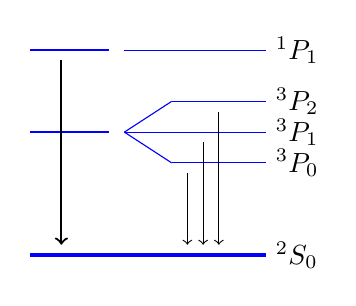
\begin{tikzpicture}[xscale=2,yscale =1.3]
      % levels
      \draw [ultra thick,blue] (0,-0.5) -- (1.5,-0.5);
      \draw [thick,blue] (0,0.7) -- (0.5,0.7);
      \draw [thick,blue] (0,1.5) -- (0.5,1.5);
      \draw [thin,blue] (0.6,1.5) -- (1.5,1.5);
      \draw [thin,blue] (0.6,0.7) -- (0.9,0.7);
      \draw [thin,blue] (0.6,0.7) -- (0.9,1);
      \draw [thin,blue] (0.6,0.7) -- (0.9,0.4);
      \draw [thin,blue] (0.9,0.7) -- (1.5,0.7);
      \draw [thin,blue] (0.9,0.4) -- (1.5,0.4);
      \draw [thin,blue] (0.9,1) -- (1.5,1);
      \draw node [right] at (1.5,1.5) {${}^1P_{1}$};
      \draw node [right] at (1.5,1) {${}^3P_{2}$};
      \draw node [right] at (1.5,0.7) {${}^3P_{1}$};
      \draw node [right] at (1.5,0.4) {${}^3P_{0}$};
      \draw node [right] at (1.5,-0.5) {${}^2S_{0}$};
      % Decay lines
      \draw [thick, ->] (0.2,1.4) -- (0.2,-0.4);
      \draw [thin, ->] (1.0,0.3) -- (1.0,-0.4);
      \draw [thin, ->] (1.1,0.6) -- (1.1,-0.4);
      \draw [thin, ->] (1.2,0.9) -- (1.2,-0.4);
    \end{tikzpicture}
    \caption{Niveles de un alcalinotérreo}
    \label{fig:alcaliterlevel}
  \end{marginfigure}
\end{description}
Las configuraciones complementarias\footnote{Aquellas en las que
  faltan electrones para completar la capa, en lugar de haber sólo
  unos pocos (capas de valencia llenas a más de la mitad). Por
  ejemplo, para una capa $(np)^1$ se tiene la capa $(np)^5$. Se
  comportan de manera similar, ya que basta con escoger los números
  cuánticos de los huecos en lugar de los de los electrones.} son exactamente iguales, excepto
que cuando la $J$ disminuye la energía aumenta, como indican las
reglas de Hund.


% Use regla, not teorema
\begin{regla*}[Regla del intervalo de Landé]
Bajo dos hipótesis
\begin{itemize}
\item $W_\text{EF}\ll W$ (acoplamiento L-S)
\item El término dominante en $W_\text{EF}$ es el de espín-órbita, $\sum f(r_i)\mathbf{l}_i \mathbf{s}_i$
\end{itemize}
Se tiene en la figura \ref{fig:landerule} que
\begin{equation}
  \frac{E(LS,J+2)-E(LS,J+1)}{E(LS,J+1)-E(LS,J)} = \frac{J+2}{J+1}
\end{equation}
\end{regla*}
\begin{marginfigure}
    \centering
    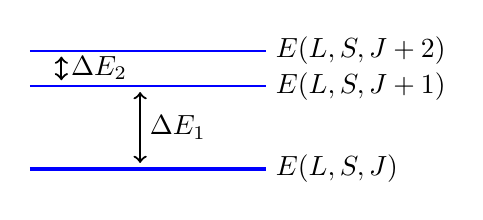
\begin{tikzpicture}[xscale=2,yscale =1.5]
      % levels
      \draw [ultra thick,blue] (0,0) -- (1.5,0);
      \draw [thick,blue] (0,0.7) -- (1.5,0.7);
      \draw [thick,blue] (0,1.0) -- (1.5,1.0);
      \draw node [right] at (1.5,1.0) {$E(L,S,J+2)$};
      \draw node [right] at (1.5,0.7) {$E(L,S,J+1)$};
      \draw node [right] at (1.5,0) {$E(L,S,J)$};
      % ΔE lines
      \draw [thick, <->] (0.2,0.75) -- (0.2,0.95);
      \draw [thick, <->] (0.7,0.65) -- (0.7,0.05);
      \draw node [right] at (0.2,0.85) {$\Delta E_2$};
      \draw node [right] at (0.7,0.35) {$\Delta E_1$};
    \end{tikzpicture}
    \caption{Regla de Landé. El cociente entre las energías es $\frac{J+2}{J+1}$.}
    \label{fig:landerule}
  \end{marginfigure}

Esta regla es la razón de ser histórica del subíndice $a$ en los términos
espectroscópicos como ${}^3 P_a$. Se utilizaba $a$ como marcador de la distancia
entre niveles, pero era un indicador del momento angular total aunque
no se supiera.
La regla funciona bien hasta el germanio aproximadamente, luego se rompe la
primera hipótesis\footnote{Para $Z>30$ se pasa de acoplamiento L-S a acoplamiento
j-j.}.

\subsection{Reglas de selección $\varepsilon_1$}
Para averiguar las reglas de selección del dipolo eléctrico
($\varepsilon_1$) suponemos acoplamiento LS. Comenzamos por sustituir
el operador tensorial ya visto por una suma a todos los átomos,

\begin{equation}
  \mathbf{r} \ \rightarrow \ \sum_{i=1}^Z \mathbf{r}_i
\end{equation}

La probabilidad de transición será

\begin{equation}
  \Lambda_{if} = \frac{4}{3}\frac{\omega^3}{c^2}\alpha
  \abs{\matrixel{ (\alpha LSJM)_f}{\textstyle \sum_{i}\mathbf{r}_i}{(\alpha LSJM)_i}
}^2
 \label{eq:foobar}
\end{equation}
donde $f$ tiene el significado de final e $i$ de inicial. 

La primera regla de selección no tiene nada que ver con el teorema de
Wigner-Eckart. Se tiene que $\sum_{i}\mathbf{r}_i=\boldrm{R}$ es impar, por lo que la
paridad a ambos lados del elemento de matriz de \eqref{eq:foobar} debe ser
contraria\footnote{Si no es así obtendremos para la integral una
  ecuación del estilo $I=-I$, y por tanto necesariamente $I=0$, lo
  cual se quiere evitar.}.

Notar que la paridad de $(1s)^2,(2s)^2,\cdots,(n\ell)^k$ depende
únicamente de los armónicos esféricos, por lo que depende de
$(-1)^{\ell_1},\cdots,(-1)^{\ell_z}$; las capas completas tienen
paridad positiva\footnote{
  Se tiene $(nl)^{2(2\ell+1)}$, luego (+1).
}.

Desarrollando \eqref{eq:foobar} obtenemos
\begin{equation}
  \begin{split}
    \mel{F}{\boldrm{R}}{I} &= \sum_{\bigstar}
    (LSM_LM_S|JM)_f^*(LSM_LM_S|JM)_i \times \\
    &\times \mel{(\alpha L M_L)_f}{\boldrm{R}}{(\alpha L M_L)_i} \cdot
    \braket{(\alpha S M_S)_f}{(\alpha S M_S)_i}
  \end{split}
\end{equation}
donde el sumatorio se extiende sobre $\bigstar =
\{(M_LM_S)_f\}\cup\{(M_LM_S)_i\}$. Se ha realizado un desacoplo de la
función de ondas, lo que nos da varios coeficientes de Clebsch-Gordan.
Forzar que $\mel{F}{\boldrm{R}}{I}\neq 0$ nos da varias reglas, junto
a la obtenida para la paridad $P$:
\begin{mdframed}
\begin{enumerate}
\item $J_f\in J_i\otimes 1$
\item $P_f \neq P_i$
\item $S_f = S_i$. Esta regla no se cumple cuando aparecen las \emph{líneas
  de intercombinación}, no contempladas en la aproximación LS. 

Implica
que no hay transiciones de singlete a triplete.
\item $L_f\in L_i\otimes 1$
\item La configuración final se diferencia de la inicial en un sólo
  electrón, el que ``salta''.
\end{enumerate}
\end{mdframed}

Combinando las reglas para $P$ y $L$ se obtiene que $|\Delta\ell|=1$.

%%% Local Variables:
%%% mode: latex
%%% TeX-master: "../resumen"
%%% End:
